\section{Matrices Suite} \label{matricesSuite}





\subsection*{Preliminary Set}
This short report shows the preliminary set of matrices to use beside the performance results of the second shared memory version. In this version, the communication is theoretically between nodes. Since here we are only using one node, the performance shown must be very similar to the report produced for the first shared memory version.

UPDATE: This results were produced after allowing vectorization in the spmv function. The results are puzzling because, while for one process the intel compiler gets a boost, the Gnu compiler gets a slowdown. The pgi compiler gets a large boost for some matrices and slowdown for others.

\medskip

\begin{comment}
\subsection*{Organization}


\medskip

The lessons learned during the development of this work will be remarked and commented in the coming sections. This document is organized as follows:

\begin{itemize} 
\item Section 2 describes a small set of functions and techniques required to use MPI$_{sm}$ as a shared memory and as a hybrid programming model.

\item Section 3 describes some technical aspects that affect the performance of both MPI$_{sm}$ and OpenMP.

\item Section 4 presents and compares the performance of two versions of a program conforming to the shared memory programming model (OpenMP Vs. MPI$_{sm}$)

\item Section 5 compares the performance of a traditional and a hybrid (MPI+MPI$_{sm}$) parallel implementation of the sparse matrix-vector multiplication (SPMV) kernel.

\item Section 6 contains a brief summary and some conclusions.


\end{itemize}

\end{comment}



\begin{figure} [ht!]
    \centering
    \captionsetup{justification=centering, singlelinecheck=false}
    \begin{subfigure}{.65\textwidth}
      \centering
      \hspace*{-3.5cm} 
      \includegraphics[width=0.95\linewidth]{../../matrices/atmosmodm.png}
      %\caption[]{Matrix}
      \label{fig:atmosmodm_matrix}
    \end{subfigure}%
    \begin{subfigure}{.65\textwidth}
      \centering
      \hspace*{-6.0cm} 
      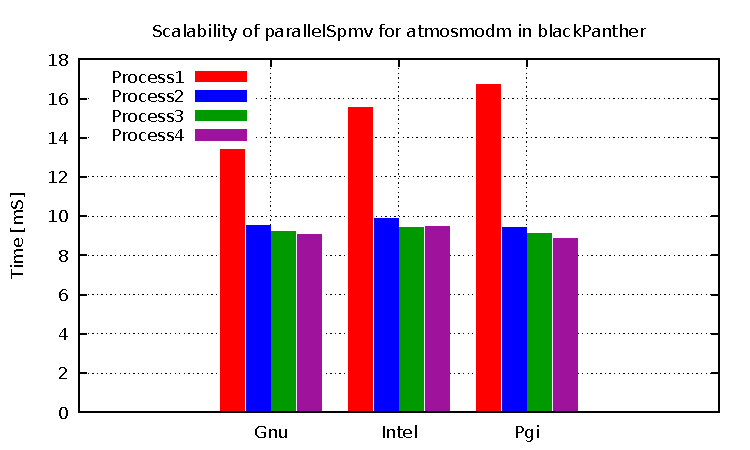
\includegraphics[page=1, width=0.95\linewidth]{../plots/blackPanther.pdf}
      %\caption{Performance.}
      \label{fig:atmosmodm_performance}
    \end{subfigure}
\caption{Matrix: atmosmodm}
\label{fig:atmosmodm}
\end{figure}

\begin{figure} [ht!]
    \centering
    \captionsetup{justification=centering, singlelinecheck=false}
    \begin{subfigure}{.65\textwidth}
      \centering
      \hspace*{-3.5cm} 
      \includegraphics[width=0.95\linewidth]{../../matrices/crankseg_1.png}
      %\caption[]{Matrix}
      \label{fig:crankseg_1_matrix}
    \end{subfigure}%
    \begin{subfigure}{.65\textwidth}
      \centering
      \hspace*{-6.0cm} 
      \includegraphics[page=2, width=0.95\linewidth]{../plots/blackPanther.pdf}
      %\caption{Performance.}
      \label{fig:crankseg_1_performance}
    \end{subfigure}
\caption{Matrix: crankseg\_1}
\label{fig:crankseg_1}
\end{figure}

\begin{figure} [ht!]
    \centering
    \captionsetup{justification=centering, singlelinecheck=false}
    \begin{subfigure}{.65\textwidth}
      \centering
      \hspace*{-3.5cm} 
      \includegraphics[width=0.95\linewidth]{../../matrices/Freescale1.png}
      %\caption[]{Matrix}
      \label{fig:Freescale1_matrix}
    \end{subfigure}%
    \begin{subfigure}{.65\textwidth}
      \centering
      \hspace*{-6.0cm} 
      \includegraphics[page=3, width=0.95\linewidth]{../plots/blackPanther.pdf}
      %\caption{Performance.}
      \label{fig:Freescale1_performance}
    \end{subfigure}
\caption{Matrix: Freescale1}
\label{fig:Freescale1}
\end{figure}

\begin{figure} [ht!]
    \centering
    \captionsetup{justification=centering, singlelinecheck=false}
    \begin{subfigure}{.65\textwidth}
      \centering
      \hspace*{-3.5cm} 
      \includegraphics[width=0.95\linewidth]{../../matrices/parabolic_fem.png}
      %\caption[]{Matrix}
      \label{fig:parabolic_fem_matrix}
    \end{subfigure}%
    \begin{subfigure}{.65\textwidth}
      \centering
      \hspace*{-6.0cm} 
      \includegraphics[page=4, width=0.95\linewidth]{../plots/blackPanther.pdf}
      %\caption{Performance.}
      \label{fig:parabolic_fem_performance}
    \end{subfigure}
\caption{Matrix: parabolic\_fem}
\label{fig:parabolic_fem}
\end{figure}

\begin{figure} [ht!]
    \centering
    \captionsetup{justification=centering, singlelinecheck=false}
    \begin{subfigure}{.65\textwidth}
      \centering
      \hspace*{-3.5cm} 
      \includegraphics[width=0.95\linewidth]{../../matrices/rajat30.png}
      %\caption[]{Matrix}
      \label{fig:rajat30_matrix}
    \end{subfigure}%
    \begin{subfigure}{.65\textwidth}
      \centering
      \hspace*{-6.0cm} 
      \includegraphics[page=5, width=0.95\linewidth]{../plots/blackPanther.pdf}
      %\caption{Performance.}
      \label{fig:rajat30_performance}
    \end{subfigure}
\caption{Matrix: rajat30}
\label{fig:rajat30}
\end{figure}


\begin{figure} [ht!]
    \centering
    \captionsetup{justification=centering, singlelinecheck=false}
    \begin{subfigure}{.65\textwidth}
      \centering
      \hspace*{-3.5cm} 
      \includegraphics[width=0.95\linewidth]{../../matrices/ship_001.png}
      %\caption[]{Matrix}
      \label{fig:ship_001_matrix}
    \end{subfigure}%
    \begin{subfigure}{.65\textwidth}
      \centering
      \hspace*{-6.0cm} 
      \includegraphics[page=6, width=0.95\linewidth]{../plots/blackPanther.pdf}
      %\caption{Performance.}
      \label{fig:ship_001_performance}
    \end{subfigure}
\caption{Matrix: ship\_001}
\label{fig:ship_001}
\end{figure}

\begin{figure} [ht!]
    \centering
    \captionsetup{justification=centering, singlelinecheck=false}
    \begin{subfigure}{.65\textwidth}
      \centering
      \hspace*{-3.5cm} 
      \includegraphics[width=0.95\linewidth]{../../matrices/Si34H36.png}
      %\caption[]{Matrix}
      \label{fig:Si34H36_matrix}
    \end{subfigure}%
    \begin{subfigure}{.65\textwidth}
      \centering
      \hspace*{-6.0cm} 
      \includegraphics[page=7, width=0.95\linewidth]{../plots/blackPanther.pdf}
      %\caption{Performance.}
      \label{fig:Si34H36_performance}
    \end{subfigure}
\caption{Matrix: Si34H36}
\label{fig:Si34H36}
\end{figure}

\begin{figure} [ht!]
    \centering
    \captionsetup{justification=centering, singlelinecheck=false}
    \begin{subfigure}{.65\textwidth}
      \centering
      \hspace*{-3.5cm} 
      \includegraphics[width=0.95\linewidth]{../../matrices/stomach.png}
      %\caption[]{Matrix}
      \label{fig:stomach_matrix}
    \end{subfigure}%
    \begin{subfigure}{.65\textwidth}
      \centering
      \hspace*{-6.0cm} 
      \includegraphics[page=8, width=0.95\linewidth]{../plots/blackPanther.pdf}
      %\caption{Performance.}
      \label{fig:stomach_performance}
    \end{subfigure}
\caption{Matrix: stomach}
\label{fig:stomach}
\end{figure}

\begin{figure} [ht!]
    \centering
    \captionsetup{justification=centering, singlelinecheck=false}
    \begin{subfigure}{.65\textwidth}
      \centering
      \hspace*{-3.5cm} 
      \includegraphics[width=0.95\linewidth]{../../matrices/Transport.png}
      %\caption[]{Matrix}
      \label{fig:Transport_matrix}
    \end{subfigure}%
    \begin{subfigure}{.65\textwidth}
      \centering
      \hspace*{-6.0cm} 
      \includegraphics[page=9, width=0.95\linewidth]{../plots/blackPanther.pdf}
      %\caption{Performance.}
      \label{fig:Transport_performance}
    \end{subfigure}
\caption{Matrix: Transport}
\label{fig:Transport}
\end{figure}


\medskip
